% AIS-SPRT: SDN course project paper, IEEE conference template (IEEEtran).
% Figures and generated/results.tex are produced by scripts/eval_detectors.py and reports/build_ieee_report.py.
\documentclass[conference]{IEEEtran}
\IEEEoverridecommandlockouts
\usepackage{cite}
\usepackage{amsmath,amssymb,amsfonts,amsthm}
\usepackage{algorithm}
\usepackage{algpseudocode}
\usepackage{graphicx}
\usepackage{textcomp}
\usepackage{xcolor}
\usepackage{booktabs}
\usepackage{array}
\usepackage{multirow}
\usepackage{tikz}
\usetikzlibrary{arrows.meta,positioning,automata}
\usepackage{url}
\usepackage[hidelinks]{hyperref}
\usepackage{placeins}
\renewcommand{\topfraction}{0.92}\renewcommand{\bottomfraction}{0.8}\renewcommand{\textfraction}{0.05}
\renewcommand{\floatpagefraction}{0.75}\renewcommand{\dbltopfraction}{0.95}\renewcommand{\dblfloatpagefraction}{0.75}
\newtheorem{proposition}{Proposition}
\newtheorem{definition}{Definition}
% generated by scripts/gen_results_tex.py -- do not edit
\newcommand{\SlowLimit}{215}
\newcommand{\SlowRate}{0.0046}
\newcommand{\NRuns}{24}
\newcommand{\NTest}{16}
\newcommand{\NPkts}{368\,633}
\newcommand{\NAttempts}{44\,855}
\newcommand{\OursTPR}{1.000}
\newcommand{\OursFPR}{0.000}
\newcommand{\OursFone}{1.000}
\newcommand{\OursPrec}{1.000}
\newcommand{\OursFP}{0}
\newcommand{\OursTP}{16}
\newcommand{\OursP}{16}
\newcommand{\OursN}{176}
\newcommand{\OursDelay}{3.07}
\newcommand{\TRWTPR}{0.875}
\newcommand{\TRWFPR}{0.006}
\newcommand{\TRWFone}{0.903}
\newcommand{\TRWPrec}{0.933}
\newcommand{\TRWFP}{1}
\newcommand{\TRWTP}{14}
\newcommand{\TRWP}{16}
\newcommand{\TRWN}{176}
\newcommand{\TRWDelay}{3.57}
\newcommand{\IATPR}{0.125}
\newcommand{\IAFPR}{0.000}
\newcommand{\IAFone}{0.222}
\newcommand{\IAPrec}{1.000}
\newcommand{\IAFP}{0}
\newcommand{\IATP}{2}
\newcommand{\IAP}{16}
\newcommand{\IAN}{176}
\newcommand{\IADelay}{0.07}
\newcommand{\NaiveTPR}{0.125}
\newcommand{\NaiveFPR}{0.000}
\newcommand{\NaiveFone}{0.222}
\newcommand{\NaivePrec}{1.000}
\newcommand{\NaiveFP}{0}
\newcommand{\NaiveTP}{2}
\newcommand{\NaiveP}{16}
\newcommand{\NaiveN}{176}
\newcommand{\NaiveDelay}{0.07}
\newcommand{\EntTPR}{0.875}
\newcommand{\EntFPR}{0.193}
\newcommand{\EntFone}{0.438}
\newcommand{\EntPrec}{0.292}
\newcommand{\EntFP}{34}
\newcommand{\EntTP}{14}
\newcommand{\EntP}{16}
\newcommand{\EntN}{176}
\newcommand{\EntDelay}{4.73}
\newcommand{\RFTPR}{0.750}
\newcommand{\RFFPR}{0.182}
\newcommand{\RFFone}{0.400}
\newcommand{\RFPrec}{0.273}
\newcommand{\RFFP}{32}
\newcommand{\RFTP}{12}
\newcommand{\RFP}{16}
\newcommand{\RFN}{176}
\newcommand{\RFDelay}{10.05}
\newcommand{\OverallRows}{\textbf{AIS-SPRT (ours)} & \textbf{1.000} & \textbf{0.000} & \textbf{1.000} & \textbf{1.000} & \textbf{3.07} \\
TRW & 0.875 & 0.006 & 0.933 & 0.903 & 3.57 \\
IA-Window & 0.125 & 0.000 & 1.000 & 0.222 & 0.07 \\
Naive-Window & 0.125 & 0.000 & 1.000 & 0.222 & 0.07 \\
Entropy & 0.875 & 0.193 & 0.292 & 0.438 & 4.73 \\
Random Forest & 0.750 & 0.182 & 0.273 & 0.400 & 10.05 \\}

%% generated by scripts/eval_cicids.py
\newcommand{\cicPackets}{9{,}915{,}680}
\newcommand{\cicAttempts}{396{,}429}
\newcommand{\cicCalAttempts}{95{,}334}
\newcommand{\cicTestAttempts}{301{,}095}
\newcommand{\cicNeg}{8}
\newcommand{\cicH}{620}
\newcommand{\cicSmax}{513}
\newcommand{\cicRows}{\textbf{AIS-SPRT} & 2/2 & 2/8 & 0.667 & 45.5 & 31.8 \\
TRW & 1/2 & 2/8 & 0.400 & 45.5 & -- \\
Entropy & 1/2 & 0/8 & 0.667 & 45.5 & -- \\
Random Forest & 2/2 & 5/8 & 0.444 & 0.0 & 60.0 \\
Isolation Forest & 1/2 & 1/8 & 0.500 & 50.0 & -- \\
IA-Window & 1/2 & 0/8 & 0.667 & 45.5 & -- \\
Naive-Window & 1/2 & 2/8 & 0.400 & 45.5 & -- \\}
\newcommand{\swCicAFone}{0.80}\newcommand{\swCicAFP}{1}\newcommand{\swCicADelay}{45.5}
\newcommand{\swEmuAFone}{1.00}\newcommand{\swEmuAFP}{0}\newcommand{\swEmuADelay}{4.6}
\newcommand{\swCicBFone}{1.00}\newcommand{\swCicBFP}{0}\newcommand{\swCicBDelay}{45.5}
\newcommand{\swEmuBFone}{0.97}\newcommand{\swEmuBFP}{0}\newcommand{\swEmuBDelay}{6.1}
\newcommand{\cicOursTP}{2}\newcommand{\cicOursFP}{2}\newcommand{\cicOursCalFP}{0}
\newcommand{\cicEmuHTP}{2}\newcommand{\cicEmuHFP}{5}\newcommand{\cicEmuHCalFP}{5}
\newcommand{\cicNoNovTP}{2}\newcommand{\cicNoNovFP}{2}\newcommand{\cicNoNovCalFP}{0}
\newcommand{\cicNoCusTP}{1}\newcommand{\cicNoCusFP}{2}\newcommand{\cicNoCusCalFP}{0}
\newcommand{\cicNoDecayTP}{2}\newcommand{\cicNoDecayFP}{2}\newcommand{\cicNoDecayCalFP}{2}
\newcommand{\cicRescoreTP}{2}\newcommand{\cicRescoreFP}{2}\newcommand{\cicRescoreCalFP}{0}

\newcommand{\cmd}[1]{\texttt{#1}}

\renewcommand{\topfraction}{0.92}\renewcommand{\bottomfraction}{0.6}\renewcommand{\textfraction}{0.08}
\renewcommand{\floatpagefraction}{0.85}\renewcommand{\dbltopfraction}{0.92}\renewcommand{\dblfloatpagefraction}{0.85}
\setcounter{topnumber}{3}\setcounter{totalnumber}{5}\setcounter{dbltopnumber}{2}
\setlength{\textfloatsep}{8pt plus 2pt minus 2pt}\setlength{\floatsep}{6pt plus 2pt minus 2pt}
\setlength{\dbltextfloatsep}{8pt plus 2pt minus 2pt}\setlength{\abovecaptionskip}{3pt}
\begin{document}

\title{SDN-Based Network Traffic Monitor and Anomaly Detection:\\ Initiation-Aware Sequential Detection with Graded OpenFlow Mitigation}

\author{
\IEEEauthorblockN{Gagan Rathod}
\IEEEauthorblockA{23bcs106}
\and
\IEEEauthorblockN{Atulesh Sahoo}
\IEEEauthorblockA{23bcs022}
\and
\IEEEauthorblockN{Ganesh Daware}
\IEEEauthorblockA{23bcs038}
\and
\IEEEauthorblockN{Bhagya Vishwakarma}
\IEEEauthorblockA{23bcs029}
\and
\IEEEauthorblockN{Dudlewar Adinath}
\IEEEauthorblockA{23bcs046}
\and
\IEEEauthorblockN{Harshit}
\IEEEauthorblockA{23bcs037}
\and
\IEEEauthorblockA{\textit{Department of Computer Science and Engineering}\\
\textit{Indian Institute of Information Technology Dharwad}, Dharwad, Karnataka, India}
}

\maketitle

\begin{abstract}
When a network monitor drives a Software-Defined Networking (SDN) controller, every detection becomes an enforcement
action: the detector must not block legitimate hosts, must catch deliberately slow scanners and must react in proportion
to its evidence. We present \emph{AIS-SPRT}, an initiation-aware sequential probability ratio test that scores each host by
the \emph{outcome} of the first contacts it \emph{initiates}, weights failures by the novelty of the target and lets evidence
decay, with a CUSUM test for floods. Its decisions drive a \emph{graded} OpenFlow response (path block, host block,
exponential back-off, race-free installation). We derive error bounds and the slowest detectable scan rate in closed form.
On \NRuns{} labelled recordings of an emulated 16-host campus network with slow, horizontal, distributed and flood attacks
and a server outage, AIS-SPRT detected every attacker without flagging any benign host (F1 \OursFone{}), against
\TRWFone{} for Threshold Random Walk (TRW), \EntFone{} for entropy, \RFFone{} for a Random Forest and \IAFone{} for window
detectors. On the public CIC-IDS2017 capture (\cicPackets{} packets), without re-tuning the scan test, it was the only
detector besides the Random Forest to catch both the port scan and the DDoS, with fewer false alarms, and reached F1
\swCicBFone{} at a stricter false-alarm target where TRW stayed at or below 0.50. A live Mininet/POX loop blocked
attackers within 1.4~s.
\end{abstract}

\begin{IEEEkeywords}
Software-defined networking, OpenFlow, port scan detection, sequential hypothesis testing, SPRT, CUSUM, intrusion
prevention, graded mitigation, Mininet.
\end{IEEEkeywords}

% =====================================================================================================
\section{Introduction}
Port scanning is the reconnaissance step that precedes most intrusions~\cite{bhuyan2014anomaly,pittman2023ml}. In
Software-Defined Networking (SDN) a logically centralised controller can install a drop rule on every switch within
milliseconds~\cite{mckeown2008openflow,kreutz2015sdn}, which makes automatic blocking attractive and dangerous at once: a
false positive now disconnects a legitimate host, and an attacker who knows the detector can trigger it against a
victim~\cite{hong2015poisoning,scotthayward2016survey}.

Most SDN detection pipelines count per-source features in fixed windows (new flows, distinct ports, entropy) and compare
them with thresholds or feed them to a classifier~\cite{braga2010lightweight,giotis2014combining,tang2016deep,belachew2025robust}.
When they drive blocking, they show three weaknesses. (i)~\emph{Role confusion}: counting all new flows does not separate a
host that \emph{opens} many connections from one that \emph{answers} many, so busy servers and multi-service clients look
like scanners. (ii)~\emph{A rate floor}: a window of $W$ seconds and a threshold of $\theta$ ports cannot see a scanner
slower than $\theta/W$ probes per second~\cite{ring2018slow}. (iii)~\emph{Disproportionate response}: one threshold crossing
blocks the whole host for a fixed time, and the rule-installation sequence has a race in which a newly learned forwarding
entry can outrank the drop rule.

\subsection*{Problem statement}
Given the mirrored traffic of an SDN and a controller that programs every switch, decide online and without training data
whether each host is scanning or flooding, and block it automatically such that (P1)~legitimate hosts are not blocked,
including busy servers, multi-service clients and clients of a service that is down; (P2)~slow, horizontal and
distributed scans and floods are detected; and (P3)~the response is proportionate, escalates for repeat offenders and
cannot be bypassed during rule installation. Window detectors violate P1 and P2; fixed whole-host blocking violates P3.

\subsection*{Proposed solution}
Legitimate clients mostly reach services that exist, so their attempts succeed; scanners probe services that do not exist,
so theirs fail. We therefore score each host sequentially by the outcomes of the connections it \emph{initiates}, scoring
each service once, discounting failures on services that many hosts use (outages are not attacks) and letting old evidence
fade, and add a CUSUM test for floods, whose attempts succeed. Decisions drive a graded, race-free OpenFlow response.

Our contributions are:
\begin{enumerate}
\item \textbf{AIS-SPRT} (Section~\ref{sec:method}), which extends Threshold Random Walk~\cite{jung2004trw} with
novelty-weighted evidence and evidence decay and pairs it with a CUSUM~\cite{page1954cusum} flood test, with closed-form
error bounds and the slowest detectable scan rate (Proposition~\ref{prop:rate}).
\item A \textbf{graded OpenFlow mitigation} policy (Section~\ref{sec:mitig}): path block at suspicion, host block at
decision, exponential back-off and a packet-in guard that closes the installation race.
\item An \textbf{evaluation} (Section~\ref{sec:eval}) on \NRuns{} labelled recordings of a 16-host emulated campus network
against five baselines, with ROC curves, delay and ablation, and a \textbf{cross-dataset test on the public CIC-IDS2017}
capture with seven detectors, including two machine-learning models.
\item A \textbf{working closed loop} in Mininet, Open vSwitch and POX.
\end{enumerate}

% =====================================================================================================
\section{Related Work}\label{sec:related}
\begin{table*}[!t]
\caption{Comparison with representative detection approaches}\label{tab:related}
\centering\footnotesize
\resizebox{\textwidth}{!}{%
\begin{tabular}{@{}lllllll@{}}
\toprule
Approach & Input & Decision & Slow scans & Benign multi-port & Error control & Response \\
\midrule
Threshold / window~\cite{roesch1999snort,paxson1999bro} & packets or flows & count $>\theta$ & no (rate floor) & flagged & none & alert or block \\
Entropy~\cite{lakhina2005mining,giotis2014combining} & flow features & entropy shift & no & flagged & none & block \\
TRW~\cite{jung2004trw,mehdi2011revisiting} & first-contact outcomes & SPRT & yes & not flagged & $\alpha,\beta$ & alert \\
ML / DL~\cite{braga2010lightweight,tang2016deep,belachew2025robust,benlloch2026mldas} & flow features & classifier & data-dependent & data-dependent & none & block \\
In-switch~\cite{krack2025portest,karrakchou2025collaborative} & counters / sketches & threshold / NN & limited & flagged & none & drop \\
\textbf{AIS-SPRT (ours)} & initiated-attempt outcomes & weighted SPRT+CUSUM & yes (Prop.~\ref{prop:rate}) & not flagged & $\alpha,\beta$ & graded \\
\bottomrule
\end{tabular}}
\end{table*}
\subsection{Security in software-defined networks}
SDN separates the control plane from the data plane and exposes the forwarding state of every switch to a logically
centralised controller through OpenFlow~\cite{mckeown2008openflow,onf2009of10}. Kreutz~\emph{et al.} survey the
architecture and its research challenges~\cite{kreutz2015sdn}, and Scott-Hayward~\emph{et al.} review the security
implications in both directions: SDN as a tool for security, and the security of the SDN itself~\cite{scotthayward2016survey}.
The same centralisation that enables network-wide reaction creates new attack surfaces. AVANT-GUARD protects the control
plane against saturation by SYN floods~\cite{shin2013avantguard}, SPHINX detects attacks on network topology and data-plane
forwarding by checking flow-graph invariants~\cite{dhawan2015sphinx}, and Hong~\emph{et al.} show that topology
information can be poisoned by forged LLDP messages and host migrations~\cite{hong2015poisoning}. FRESCO provides a
framework in which security applications are composed from modules and their decisions are translated into flow
rules~\cite{shin2013fresco}. For distributed denial of service, Yan~\emph{et al.} discuss how SDN changes both the attack
and the defence in cloud environments~\cite{yan2016ddos}. More recently, Janabi~\emph{et al.} survey intrusion detection
systems for SDN and classify them by detection technique, placement and evaluation data~\cite{janabi2024survey}, and
Wainwright~\emph{et al.} review SDN security detection strategies with a focus on the constraints of small and medium-sized
enterprises~\cite{wainwright2025sdn}. A recurring observation in these surveys is that detection accuracy is reported far
more often than the consequences of acting on a detection, which is the gap our graded mitigation targets.

\subsection{Port-scan detection}
Classical intrusion detection systems detect scans from a mirror port. Snort matches packets against signatures and
counts connection attempts per source~\cite{roesch1999snort}; Bro/Zeek turns traffic into events and lets policy scripts
count failed connections~\cite{paxson1999bro}. Both rely on thresholds over time windows, which trades sensitivity to slow
scans against false alarms. Jung~\emph{et al.} replaced counting by sequential hypothesis testing: Threshold Random Walk
(TRW) observes whether a host's first-contact connection attempts succeed or fail and applies Wald's sequential probability
ratio test~\cite{wald1945sequential}, detecting scanners in four or five attempts with bounded error
probabilities~\cite{jung2004trw}. Lakhina~\emph{et al.} detect scans and other anomalies network-wide from changes in the
entropy of traffic feature distributions~\cite{lakhina2005mining}. Ring~\emph{et al.} target slow scans in flow-based
traffic with an unsupervised sequential method and a supervised classifier over time windows, and report fewer false
alarms than earlier algorithms on the CIDDS-001 data set~\cite{ring2018slow}. Pittman's systematic review of machine
learning for port scans finds a small literature dominated by supervised classifiers on public data sets and warns about
reproducibility~\cite{pittman2023ml}. Within SDN, Mehdi~\emph{et al.} implemented TRW, rate limiting and other
detectors as NOX applications for home networks~\cite{mehdi2011revisiting}. Detection has also moved into the switches:
the review by Singh~\emph{et al.} systematises security applications built on programmable (P4) data
planes~\cite{singh2025programmable}, and Krack and Zitterbart detect horizontal and vertical scans on
\emph{non}-programmable switches by installing a constant number of randomised TCAM rules and reading their counters,
without mirroring~\cite{krack2025portest}. These in-switch methods are attractive for line rate, but they estimate the
\emph{number} of probes and cannot observe their \emph{outcomes}. AIS-SPRT works on the outcomes, which is what lets it
separate a monitoring agent that touches many ports successfully from a scanner that mostly fails.

\subsection{Machine learning for SDN attack detection}
Learning-based detectors dominate recent SDN security work. Braga~\emph{et al.} used self-organising maps on flow
statistics collected by NOX~\cite{braga2010lightweight}, Giotis~\emph{et al.} combined sFlow sampling with entropy-based
detection and OpenFlow mitigation~\cite{giotis2014combining}, and Tang~\emph{et al.} applied a deep neural network to
flow features~\cite{tang2016deep}. Systematic reviews by Bahashwan~\emph{et al.}~\cite{bahashwan2023systematic}, Ganeshan
and Ramasamy~\cite{ganeshan2026systematic} and Polat~\emph{et al.}~\cite{polat2026supervised} cover dozens of such
studies; they report very high accuracies, mostly on public data sets such as CIC-IDS2017~\cite{sharafaldin2018cicids}
and the SDN-specific InSDN~\cite{elsayed2020insdn}, and they repeatedly note that evaluation is offline, that class
balance and feature leakage inflate results, and that deployment in the control loop is rarely measured. Belachew~\emph{et
al.} deploy an XGBoost classifier at the edge of an SDN-IoT network and report near-perfect accuracy on their
data~\cite{belachew2025robust}. Benlloch~\emph{et al.} observe that no single model is best under all network conditions
and propose MLDAS, which switches between a decision tree, a random forest and other models according to the current load
in a Mininet/POX testbed~\cite{benlloch2026mldas}. Karrakchou~\emph{et al.} split the work between a P4 data plane and
an SDN controller with early-exit neural networks, so that easy decisions are made in the switch and hard ones are
escalated~\cite{karrakchou2025collaborative}. Most recently, Swileh and Zhang use port-level monitoring with zero-training
large language models to detect and mitigate DDoS in decentralised SDN~\cite{swileh2025proactive}. Sommer and Paxson
explain why such detectors are hard to operate: anomaly detection is not classification of a closed world, the cost of
errors is asymmetric, and results must be interpretable to be acted upon~\cite{sommer2010closed}. A classifier score does
not tell an operator how confident the decision is in a statistical sense, how it will behave on a host it has not seen,
or why a particular host was blocked. AIS-SPRT is deliberately model-based: its two error probabilities are parameters
with an explicit meaning, it needs no training data, and every decision can be explained by the sequence of failed and
successful attempts that produced it. We nevertheless include a Random Forest baseline trained on our data to compare
against a learned detector under the same conditions.

\subsection{Mitigation in the control loop}
Mitigation in SDN is usually a drop or rate-limit rule for the offending source, installed once a threshold or a
classifier fires~\cite{giotis2014combining,belachew2025robust}. Mirkovic and Reiher's taxonomy of DDoS defences already
distinguishes filtering, rate limiting and reconfiguration as responses of different strength~\cite{mirkovic2004taxonomy},
but proportionality is rarely implemented in SDN work: a single decision triggers a fixed, host-wide action. Two practical
issues are seldom discussed. First, OpenFlow~1.0 gives exact-match entries precedence over wildcard
rules~\cite{onf2009of10}, so a source-wide drop rule does not stop connections that a learning switch has already
installed; and packets that reach the controller while the drop is being installed can create new entries. Second, a
fixed block duration treats a first-time false positive and a persistent attacker identically. Our graded policy
addresses both.

\subsection{Positioning}
Table~\ref{tab:related} positions AIS-SPRT. It combines the outcome-based sequential test of
TRW~\cite{jung2004trw} with two mechanisms that matter when decisions drive blocking (novelty weighting and decay),
adds a flood test, and closes the loop with a graded, race-free OpenFlow policy.


% =====================================================================================================
\section{System and Threat Model}\label{sec:system}
The network is an OpenFlow~1.0 SDN of Open vSwitch switches under a POX controller (Fig.~\ref{fig:planes}). The core switch
mirrors all its ports to a monitoring port, so detection is out of band; a learning switch installs exact-match forwarding
entries and our component enforces mitigation and collects flow statistics. A \emph{benign} host initiates connections for a
legitimate purpose but may contact closed services (stale configuration, retries) or many services (monitoring agents). An
\emph{attacker} probes vertically, horizontally or in a distributed way, at any rate, or floods a service; it cannot spoof
replies from other hosts, and traffic between zones crosses the mirrored core.

\begin{figure}[!tb]
\centering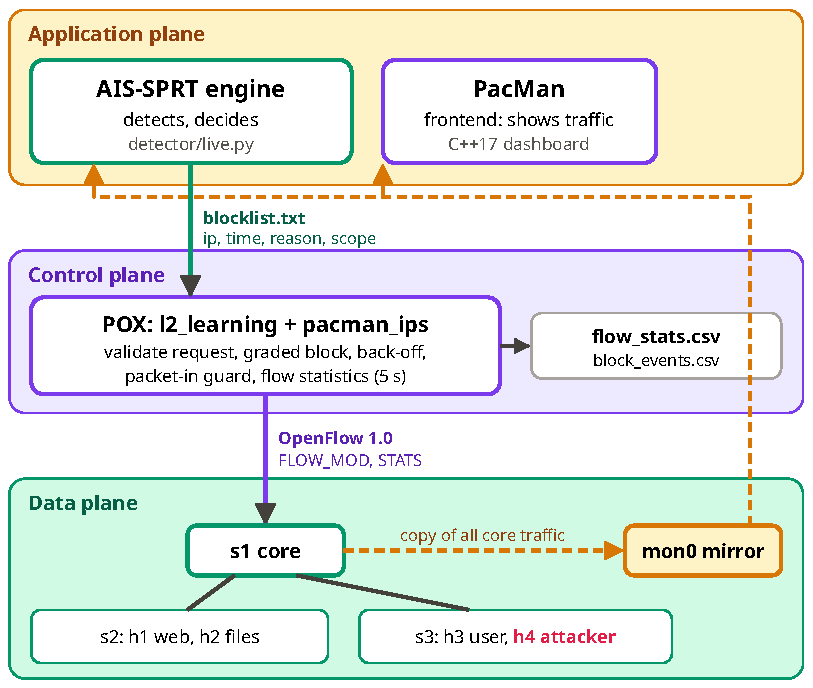
\includegraphics[width=\columnwidth]{figures/d_planes.pdf}
\caption{System architecture across the SDN planes. The detection engine watches the core mirror and sends graded
requests to the POX component, which programs every switch.}\label{fig:planes}
\end{figure}

% =====================================================================================================
\section{Traffic Monitoring}\label{sec:monitor}
The core switch mirrors every packet to \cmd{mon0}, where the engine resolves each initiated attempt into a success or a
failure and PacMan, our htop-style terminal monitor, shows the operator the same traffic (bandwidth, flows with TCP state,
host names from TLS, HTTP and DNS, alerts, active blocks); both see a copy, so monitoring adds no delay. Every 5~s the
controller also collects OpenFlow flow statistics from every switch, an independent record of what each switch forwarded or
dropped (e.g.\ the drop rule's counter on the attacker's edge switch). Packets show \emph{who initiated what and whether
it succeeded}; flow statistics show \emph{what the switches did}.

% =====================================================================================================
\section{AIS-SPRT Detection}\label{sec:method}
\subsection{Observations}
\begin{definition}[Initiated attempt]
A TCP packet with SYN set and ACK clear that opens a new 4-tuple $(s,\pi_s,d,\pi)$ is an attempt by $s$ to reach service
$(d,\pi)$; for UDP, the first datagram of a 4-tuple whose reverse direction has not been seen. The attempt's outcome
$Y\in\{0,1\}$ is $1$ (success) on a SYN-ACK or UDP reply and $0$ (failure) on RST, ICMP port-unreachable or no answer
within $T_o=3$~s.
\end{definition}
Only initiated attempts are scored, so a server's replies never count against it. Retransmitted SYNs and the mirror's
duplicate copies are ignored.

\subsection{Weighted sequential test}
Let $H_0$: $s$ is benign, $\Pr[Y=1]=\theta_0$; $H_1$: $s$ is a scanner, $\Pr[Y=1]=\theta_1$, with $\theta_1<\theta_0$
(we use $\theta_0=0.8$, $\theta_1=0.2$ as in~\cite{jung2004trw}). For each source we maintain a log-likelihood ratio
$\Lambda_s$ and update it with attempt $i$ to service $(d_i,\pi_i)$ at time $t_i$:
\begin{equation}\label{eq:update}
\Lambda_s \leftarrow \Lambda_s\, e^{-(t_i-t_{i-1})/\tau} \;+\;
\begin{cases} \ln\dfrac{\theta_1}{\theta_0}, & Y_i=1,\\[2mm] w_i\,\ln\dfrac{1-\theta_1}{1-\theta_0}, & Y_i=0,\end{cases}
\end{equation}
subject to three rules:

\emph{First-contact scoring.} As in TRW, each service $(d,\pi)$ is scored only on the first attempt of $s$ to reach it:
retries of a dead service count once, and reusing a popular service earns no repeated benign credit.

\emph{Novelty weight.} A failure is weighted by how unusual the target is:
$w_i = \max\!\big(w_{\min},\, 1/(1+n_{-s}(d_i,\pi_i))\big)$, where $n_{-s}(d,\pi)$ is the number of \emph{other} sources
that have contacted $(d,\pi)$ before: probing a port nobody uses is strong evidence ($w=1$), failing on a popular service
that is broken for everybody is weak ($w\to w_{\min}=0.25$).

\emph{Evidence decay.} $\Lambda_s$ decays towards zero with time constant $\tau=600$~s between updates, so occasional
benign failures do not accumulate over hours, while slow scans still do (Proposition~\ref{prop:rate}).

Decisions follow Wald's test~\cite{wald1945sequential} with the thresholds of~\cite{jung2004trw}:
\begin{equation}\label{eq:thresholds}
\eta_1=\ln\frac{\beta}{\alpha},\qquad \eta_0=\ln\frac{1-\beta}{1-\alpha},\qquad \eta_s=\rho\,\eta_1,
\end{equation}
where $\alpha=0.01$ is the target false-positive probability, $\beta=0.99$ the target detection probability and
$\rho=0.5$. $\Lambda_s\ge\eta_s$ raises a \emph{suspicion} (path block, Section~\ref{sec:mitig}), $\Lambda_s\ge\eta_1$ a
\emph{scanner decision} (host block), and $\Lambda_s\le\eta_0$ declares the host benign and resets $\Lambda_s$.

\begin{proposition}[Error bounds]\label{prop:bounds}
Without decay and weights ($\tau\to\infty$, $w\equiv1$), and with independent outcomes, the probability of declaring a
benign host a scanner is at most $\alpha/\beta\approx\alpha$ and the probability of missing a scanner is at most
$(1-\beta)/(1-\alpha)$~\cite{wald1945sequential}. Weights $w_i\le1$ only reduce the evidence for $H_1$, so they cannot
increase the false-positive bound.
\end{proposition}

\begin{proposition}[Slowest detectable scan]\label{prop:rate}
A scanner whose probes all fail on unused services ($w=1$) and arrive every $\Delta$ seconds is detected iff
\begin{equation}
\Delta < \tau\,\ln\!\frac{1}{1-c/\eta_1},\qquad c=\ln\frac{1-\theta_1}{1-\theta_0}.
\end{equation}
\end{proposition}
\begin{IEEEproof}
Between probes $\Lambda$ is multiplied by $q=e^{-\Delta/\tau}$ and each probe adds $c$, so after $n$ probes
$\Lambda_n=c\,(1-q^n)/(1-q)$, which increases to $c/(1-q)$. The threshold is crossed iff $c/(1-q)>\eta_1$, i.e.
$q>1-c/\eta_1$.
\end{IEEEproof}
With our parameters $c=\ln4=1.39$, $\eta_1=\ln99=4.60$ and $\tau=600$~s, the bound is $\Delta<\SlowLimit$~s: one probe
every \SlowLimit{} seconds, i.e.\ about \SlowRate{} probes per second, compared with $\theta/W=1.5$ probes per second for a
window detector with $\theta=15$, $W=10$~s. A fast scan is decided after $\lceil\eta_1/c\rceil=4$ failures, and a benign
host whose attempts fail with probability $f<0.5$ has negative expected drift $f\,c+(1-f)\ln(\theta_1/\theta_0)$.

\subsection{Flood test}
A connection flood has a high success rate and does not move $\Lambda_s$. For each source we count initiated attempts
per second, $x_k$, and run Page's one-sided CUSUM~\cite{page1954cusum}, $S_k=\max(0,S_{k-1}+x_k-\kappa)$, raising a flood
decision when $S_k>h$ ($\kappa=20$, $h=150$: a sustained excess of 20 connections per second for several seconds).

\subsection{Algorithm}
Algorithm~\ref{alg:aisprt} gives the per-attempt procedure. All state is per source or per service, and each update is
$O(1)$ amortised; the set $R$ grows with the number of distinct first contacts and can be aged out with the decay.

\begin{algorithm}[!tbp]
\caption{AIS-SPRT: per resolved initiated attempt}\label{alg:aisprt}
\begin{algorithmic}[1]
\Require attempt $(s,d,\pi,t_{\text{start}},t,Y)$; parameters $\theta_0,\theta_1,\alpha,\beta,\rho,\tau,w_{\min},\kappa,h$
\State \textbf{state:} $\Lambda_s$, $t^{\text{last}}_s$, $S_s$, $U(d,\pi)$ (users of a service), $R$ (scored first contacts), $F_s(d)$ (failures)
\State $k\gets\lfloor t_{\text{start}}\rfloor$ \Comment{flood test, one bin per second}
\If{$k\neq k_s$} \State $S_s\gets\max(0,S_s+x_s-\kappa)$; decay $S_s$ over empty bins; $k_s\gets k$; $x_s\gets0$ \EndIf
\State $x_s\gets x_s+1$
\If{$S_s+x_s-\kappa>h$} \State \textbf{emit} \textsc{Flood}$(s)$ \EndIf
\If{$(s,d,\pi)\in R$} \State $U(d,\pi)\gets U(d,\pi)\cup\{s\}$; \Return \Comment{not a first contact} \EndIf
\State $R\gets R\cup\{(s,d,\pi)\}$; \quad $n\gets|U(d,\pi)\setminus\{s\}|$; \quad $U(d,\pi)\gets U(d,\pi)\cup\{s\}$
\State $w\gets 1$ \textbf{if} $n=0$ \textbf{else} $\max(w_{\min},1/(1+n))$
\State $\Lambda_s\gets\Lambda_s\,e^{-(t-t^{\text{last}}_s)/\tau}$; \quad $t^{\text{last}}_s\gets t$
\If{$Y=1$} \State $\Lambda_s\gets\Lambda_s+\ln(\theta_1/\theta_0)$
\Else \State $\Lambda_s\gets\Lambda_s+w\ln\frac{1-\theta_1}{1-\theta_0}$; \quad $F_s(d)\gets F_s(d)+1$ \EndIf
\If{$\Lambda_s\ge\eta_1$} \State \textbf{emit} \textsc{Scanner}$(s)$; \quad $\Lambda_s\gets0$
\ElsIf{$\Lambda_s\ge\rho\,\eta_1$ \textbf{and} $s$ not suspected}
  \State \textbf{emit} \textsc{Suspect}$(s,\arg\max_d F_s(d))$; mark $s$ suspected
\ElsIf{$\Lambda_s\le\eta_0$} \State $\Lambda_s\gets0$ \Comment{benign: restart the test} \EndIf
\end{algorithmic}
\end{algorithm}

% =====================================================================================================
\section{Graded, Race-Free Mitigation}\label{sec:mitig}
Detection events reach the controller as lines \cmd{ip, time, reason, scope} in an append-only file (at most one per
source and scope every 30~s); the controller validates them (unicast, protected set, staleness) and enforces
Fig.~\ref{fig:fsm}:
\begin{itemize}
\item \textsc{Suspect}$(s,d^*)$: \emph{path block} on every switch (\cmd{nw\_src}$=s$, \cmd{nw\_dst}$=d^*$, priority
65000, drop), which protects the probable victim while $s$ keeps its other connectivity.
\item \textsc{Scanner}$(s)$ or \textsc{Flood}$(s)$: \emph{host block} for $B\cdot2^{\min(k,3)}$ seconds, $k$ = earlier
host blocks of $s$ within one hour ($B=120$~s).
\item Matching exact-match entries are deleted before the drop rule is added, because they outrank wildcard rules in
OpenFlow~1.0~\cite{onf2009of10}; a \emph{packet-in guard}, registered before the learning switch, discards packet-ins from
blocked sources so that no entry can be learned between DELETE and ADD. Blocks expire by hard timeout and are re-installed
when a switch reconnects.
\end{itemize}

\begin{figure}[!tb]
\centering
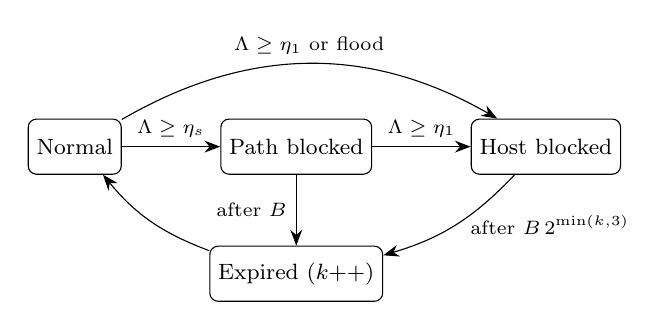
\begin{tikzpicture}[->,>={Stealth[length=2mm]},node distance=1.9cm,every state/.style={draw,rectangle,rounded corners=3pt,minimum height=7mm,font=\footnotesize,inner sep=3pt},font=\scriptsize]
\node[state] (N) {Normal};
\node[state,right=1.25cm of N] (P) {Path blocked};
\node[state,right=1.25cm of P] (H) {Host blocked};
\node[state,below=0.9cm of P] (E) {Expired ($k{+}{+}$)};
\path (N) edge node[above] {$\Lambda\ge\eta_s$} (P)
      (P) edge node[above] {$\Lambda\ge\eta_1$} (H)
      (N) edge[bend left=30] node[above] {$\Lambda\ge\eta_1$ or flood} (H)
      (H) edge[bend left=15] node[right,xshift=2pt] {after $B\,2^{\min(k,3)}$} (E)
      (P) edge node[left] {after $B$} (E)
      (E) edge[bend left=15] node[left] {} (N);
\end{tikzpicture}
\caption{Graded mitigation state machine of one source.}\label{fig:fsm}
\end{figure}

% =====================================================================================================
\section{Implementation}
The live engine (\cmd{detector/live.py}, Python) reads the mirror port through an \textsc{AF\_PACKET} socket, resolves
attempts in real time and runs Algorithm~\ref{alg:aisprt}; the same detector code is used for the offline evaluation. The
controller component (\cmd{controller/pacman\_ips.py}, POX~0.2.0, OpenFlow~1.0, 292 lines) implements Section~\ref{sec:mitig}
and also polls flow statistics from every switch. The testbed runs Mininet~2.3.1 with Open vSwitch~3.6.2 on a Fedora~43
laptop; Table~\ref{tab:params} lists all parameters.

\emph{Operator frontend.} PacMan (C++17, libpcap, FTXUI) lets an administrator see the traffic behind a decision and undo a
wrong block~\cite{sommer2010closed}; its earlier window detector is the IA-Window baseline.

\begin{table}[!tbp]
\caption{Parameters of AIS-SPRT and of the mitigation policy}\label{tab:params}
\centering\footnotesize
\setlength{\tabcolsep}{4pt}
\begin{tabular}{@{}lll@{}}
\toprule
Parameter & Value & Meaning \\
\midrule
$\theta_0$, $\theta_1$ & 0.8, 0.2 & success prob.: benign, scanner \\
$\alpha$, $\beta$ & 0.01, 0.99 & target false-pos. / detection prob. \\
$\eta_1$, $\eta_s$, $\eta_0$ & 4.60, 2.30, $-4.60$ & decision, suspicion, benign thresholds \\
$\tau$ & 600~s & evidence decay time constant \\
$w_{\min}$ & 0.25 & minimum novelty weight \\
$T_o$ & 3~s & attempt timeout (no answer = failure) \\
$\kappa$, $h$ & 20/s, 150 & CUSUM allowance, threshold$^{*}$ \\
$B$ & 120~s (live test 15~s) & base block time; back-off up to $8B$ \\
cooldown & 30~s & one request per source and scope \\
\bottomrule
\multicolumn{3}{@{}l}{\scriptsize $^{*}$$h=\cicH{}$ on CIC-IDS2017, set on benign traffic (Sec.~\ref{sec:cic}).}
\end{tabular}
\end{table}

% =====================================================================================================
\section{Evaluation}\label{sec:eval}
\subsection{Dataset}
Public SDN data sets lack connection outcomes for slow and distributed scans or are delivered as pre-computed flow
features~\cite{sharafaldin2018cicids,elsayed2020insdn}, so we recorded a labelled dataset in the emulated testbed (labels:
attacker addresses and attack start times from the schedule). The switches ran in Open vSwitch's standalone learning mode, so
the data does not depend on our controller, and the core mirror was captured with \cmd{tcpdump}. The campus network has a
core and four edge switches, four servers (10.0.0.11--14) with five TCP services each and twelve clients (10.0.0.21--32).
Benign behaviour: eleven clients send Poisson requests (0.3--3/s) to Zipf-popular servers and services, 8\% of requests go to a
closed stale service and are retried three times, and 10.0.0.21 is a monitoring agent that polls all 20 services every 5~s;
attacker hosts also run benign traffic. Eight 80~s scenarios, attacks from 20~s: \textbf{benign} only; \textbf{server
outage} (the most popular server is down for 30~s, so every client sees failures); \textbf{fast vertical} scan of 200 ports;
\textbf{slow vertical} scans at 0.5 and 0.2 probes/s; \textbf{horizontal} scan of 8 ports over 10 hosts;
\textbf{distributed} scan by three hosts at 1 probe/s each; and a \textbf{flood} of 300 attempts/s for 10~s. Three seeds
per scenario give \NRuns{} recordings, \NPkts{} packets and \NAttempts{} initiated attempts.

\subsection{Baselines and metrics}
(i)~\textbf{Naive-Window}: more than 15 distinct ports from a source to a host in 10~s, counting every new flow including
replies; (ii)~\textbf{IA-Window}: the same on initiated attempts (our previous detector); (iii)~\textbf{Entropy}: port
entropy of a source's attempts in 10~s above 3 bits; (iv)~\textbf{TRW}~\cite{jung2004trw} with the same
$\theta_0,\theta_1,\alpha,\beta$; (v)~\textbf{Random Forest} (200 trees, balanced) on six per-source window features
(attempts, distinct destinations, distinct services, failure ratio, port entropy, rate), trained on seed 1. All methods are
scored per host on seeds 2--3: an attacker alarmed after its attack starts is a true positive, any alarm for a benign host a
false positive. The parameters were fixed in advance from~\cite{jung2004trw}, except the scoring horizon (30~s re-scoring,
then first-contact scoring; both are in the ablation).

\subsection{Overall results}
Table~\ref{tab:overall} and Fig.~\ref{fig:roc} summarise the comparison. AIS-SPRT detected all 16 attacker instances of the
test seeds and flagged no benign host (F1 \OursFone{}). TRW detected every scan but missed both floods, whose attempts
succeed, and flagged one benign client during a horizontal scan (F1 \TRWFone{}). The window detectors flagged no benign host
but detected only the fast vertical scan (TPR \IATPR{}). The entropy detector flagged the monitoring agent in every test run
(FPR \EntFPR{}), and the Random Forest reached a TPR of \RFTPR{} at an FPR of \RFFPR{}, missing slow scans and the flood.
Only AIS-SPRT reaches full detection at zero false positives over a wide range of thresholds.

\begin{table}[!tbp]
\caption{Overall detection results (test seeds, all scenarios)}\label{tab:overall}
\centering\footnotesize\setlength{\tabcolsep}{3.5pt}
\begin{tabular}{@{}lrrrrr@{}}
\toprule
Method & TPR & FPR & Prec. & F1 & Delay (s) \\
\midrule
\OverallRows
\bottomrule
\end{tabular}
\end{table}

\begin{figure}[!tb]
\centering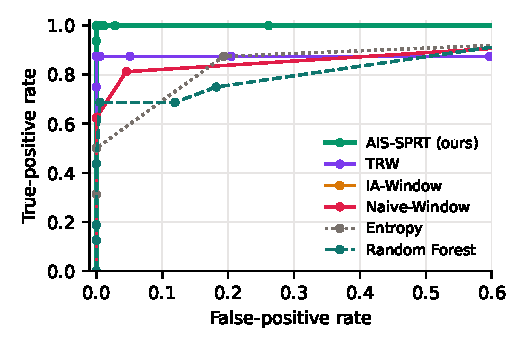
\includegraphics[width=\columnwidth]{figures/e_roc.pdf}
\caption{ROC curves obtained by sweeping each method's decision threshold (host level, test seeds).}\label{fig:roc}
\end{figure}

\subsection{Per-scenario behaviour}
\begin{figure*}[!t]
\centering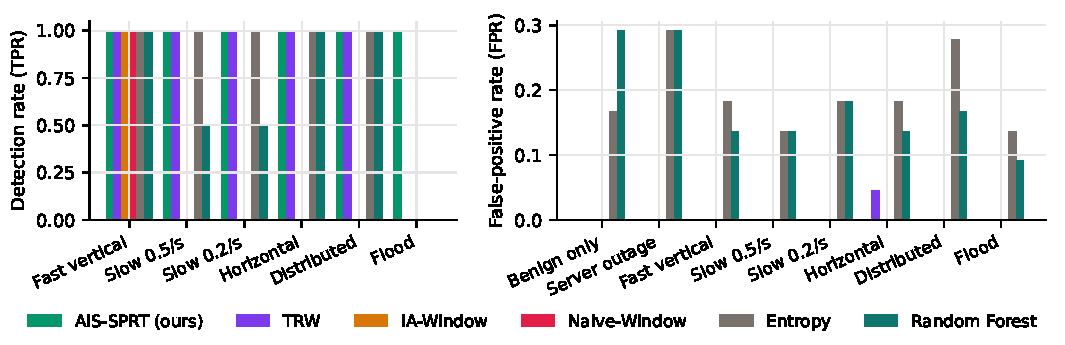
\includegraphics[width=0.9\textwidth]{figures/e_scenarios.pdf}
\caption{Detection rate (left) and false-positive rate (right) per scenario, test seeds.}\label{fig:scen}
\end{figure*}

Fig.~\ref{fig:scen} breaks the results down by scenario. Every method detects the fast vertical scan. The window detectors miss everything below 15 ports per host in 10~s (slow,
horizontal and distributed scans); AIS-SPRT and TRW detect all scans, including 0.2 probes/s, because they accumulate
evidence per probe rather than per window, and only AIS-SPRT detects the flood. In the benign and outage scenarios AIS-SPRT has
no false positive, while the entropy detector and the Random Forest flag benign hosts in every scenario, most often the
monitoring agent.

\subsection{Detection delay}
AIS-SPRT decides a fast vertical scan after a median of 0.07~s (four failed probes), a horizontal scan after 1.4~s, a
distributed scan after 4.1~s, a flood after 0.69~s and the slow scans after 19~s (0.5 probes/s) and 35~s (0.2 probes/s)
(Fig.~\ref{fig:delay}); TRW is about one second faster on slow scans because novelty weighting discounts probes to services
that the attacker's own benign traffic used. The Random Forest can only decide at the end of a 10~s window.

\begin{figure}[!tb]
\centering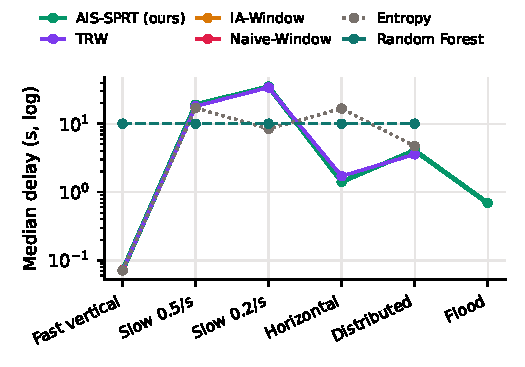
\includegraphics[width=\columnwidth]{figures/e_delay.pdf}
\caption{Median time from attack start to first alarm per scenario (log scale; missing points = not detected).}\label{fig:delay}
\end{figure}

\subsection{Ablation}
Fig.~\ref{fig:ablation} removes one mechanism at a time (all seeds). Without the novelty weight, failures on a server that
is down for everybody count fully, giving false positives in the outage and horizontal scenarios (FPR 0.008). Without the
CUSUM test the floods are lost (TPR 0.875). Re-scoring services after 30~s misses the slowest scan in two of three runs
(TPR 0.917), because the attacker's benign connections keep earning credit. Decay has no effect in 80~s recordings
($\tau=600$~s); its effect appears on the eight-hour capture of Section~\ref{sec:cic}.

\begin{figure}[!tb]
\centering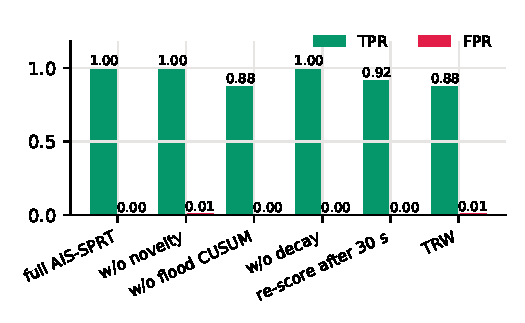
\includegraphics[width=\columnwidth]{figures/e_ablation.pdf}
\caption{Ablation: contribution of novelty weighting, the flood test, evidence decay and first-contact scoring.}\label{fig:ablation}
\end{figure}

\subsection{Graded mitigation}
For scans the path block precedes the host block (Fig.~\ref{fig:graded}) by a median of 2~s, and by 6--17~s for slow scans,
protecting the victim long before the evidence is conclusive; for fast scans both coincide, and floods go directly to a
host block.

\begin{figure}[!tb]
\centering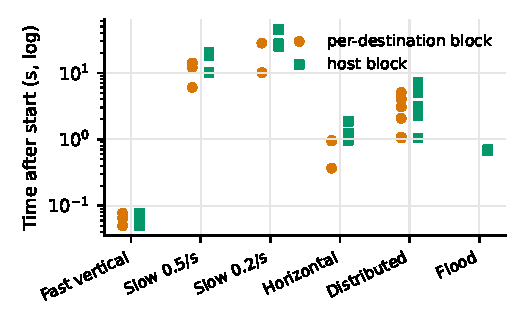
\includegraphics[width=\columnwidth]{figures/e_graded.pdf}
\caption{Time from attack start to the path block and to the host block, per attacker.}\label{fig:graded}
\end{figure}

\subsection{Cross-dataset test on CIC-IDS2017}\label{sec:cic}
We used the Friday capture of CIC-IDS2017~\cite{sharafaldin2018cicids}: \cicPackets{} packets of a real office network of
about 25 machines (09:00--17:00, \cicAttempts{} attempts) with an Nmap scan and an LOIC DDoS by 172.16.0.1 and an ARES
botnet. Attack windows come from the labelled flows, which differ from the dataset's web page~\cite{engelen2021troubleshooting}:
the scan proper (about 1000 ports) runs 14:51--15:23 after five services were probed from 13:55, and the DDoS 15:56--16:16.
Botnet hosts (command-and-control only) are excluded; the other \cicNeg{} hosts are negatives. The scan test keeps all
parameters; only the flood threshold depends on the network (real clients open 80--180 connections in a second when a page
loads), so the attack-free morning sets $h$ to 1.2 times the largest CUSUM statistic ($h=\cicH{}$) and the afternoon is the
test. The Random Forest is trained on our emulated data; an Isolation Forest~\cite{liu2008iforest} is fitted to the
morning's windows. Broadcast/multicast packets and UDP server replies do not start attempts, for every method (the emulated
results are unchanged).

\begin{table}[!tbp]
\caption{CIC-IDS2017 Friday afternoon: attacks detected, benign hosts flagged and delay}\label{tab:cic}
\centering\footnotesize\setlength{\tabcolsep}{3.2pt}
\begin{tabular}{@{}lccccc@{}}
\toprule
Method & Attacks & FP hosts & F1 & Scan (s) & DDoS (s) \\
\midrule
\cicRows
\bottomrule
\end{tabular}
\end{table}

\emph{Results.} With $\alpha=0.01$ (Table~\ref{tab:cic}) AIS-SPRT detected the scan proper after 45~s and the DDoS after
32~s, with no alarm in the morning and none for the attacker outside its attacks. It flagged two benign hosts, which TRW also
flags: a client refused by several web servers on port 80, and the DDoS victim, which sent UDP to random ports afterwards.
TRW, entropy and the window detectors miss the DDoS, whose connections succeed. The Random Forest catches both attacks but
flags five of eight benign hosts, as its features do not transfer between networks; the Isolation Forest misses the DDoS. With
the testbed $h=150$, AIS-SPRT would flag \cicEmuHFP{} hosts; without the flood test the DDoS is lost, and without decay the
morning has \cicNoDecayCalFP{} false alarms instead of \cicOursCalFP{}.

\begin{figure}[!tb]
\centering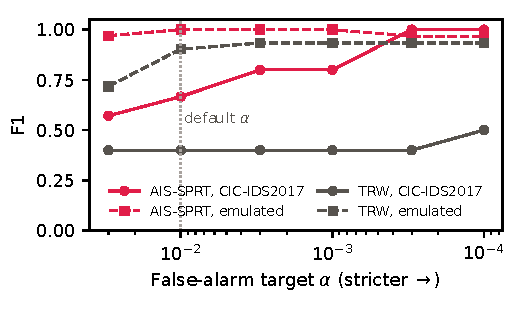
\includegraphics[width=\columnwidth]{figures/c_alpha.pdf}
\caption{F1 against the false-alarm target $\alpha$ ($\eta_1=\ln(\beta/\alpha)$) on the emulated test seeds and on
CIC-IDS2017, for AIS-SPRT and TRW.}\label{fig:alpha}
\end{figure}

\emph{Sensitivity to $\alpha$.} AIS-SPRT is above TRW at every $\alpha$ on both datasets (Fig.~\ref{fig:alpha}). On the
eight-hour capture a stricter target removes its false alarms without delaying any detection (F1 \swCicAFone{} at $10^{-3}$,
\swCicBFone{} at $3\cdot10^{-4}$), because novelty weighting and decay keep benign evidence bounded, while TRW stays at
0.40--0.50. On the emulated data $10^{-3}$ still gives F1 \swEmuAFone{} (delay \swEmuADelay{}~s) and $3\cdot10^{-4}$ starts
to miss the slowest scan, as Proposition~\ref{prop:rate} predicts; long deployments should use $\alpha\approx10^{-3}$. Scans
without SYN (FIN, Xmas, NULL) are outside the attempt model.

% written from results/aisprt_live.csv and results/aisprt_live_tests.txt (11 Nov 2026)
\subsection{Live closed loop}
On the four-host Mininet network with POX and a 15~s base block time, normal browsing produced no request. In four fast
scans of 100 ports the host block was on all three switches 0.68, 0.85, 1.05 and 1.39~s after the scan started (attacker
100\% loss, normal user 0\%). For fast scans suspicion and decision fall within milliseconds, so polling could not separate
the two stages (one of nine checks failed for this reason). Back-off gave block times of 15, 30, 60, 120 and 120~s, and a slow
scan at 0.5 probes/s was blocked on all switches after 20.2~s.


% =====================================================================================================
\section{Discussion and Limitations}
Proposition~\ref{prop:bounds} assumes independent outcomes; real outcomes are correlated (a host that is down fails every
probe), which motivates first-contact scoring and novelty weighting. A scanner that probes only services others use, or
interleaves many successes, lowers its evidence but learns little; one slower than one probe every \SlowLimit~s is missed.
Spoofed sources could abuse blocking, but a success needs a completed handshake and the first response covers one path.
The perfect emulated score shows that the mechanisms remove the baselines' failure modes, not that the detector is
error-free: on real traffic the default $\alpha$ gave two false alarms in eight hours and $h$ needed calibration. One public
day with two attacks is too few for tight confidence intervals; more data sets, larger topologies and a P4 version are
future work.

\section{Conclusion}
AIS-SPRT scores hosts by the outcomes of the connections they initiate, with novelty weighting, first-contact scoring and
decay, and drives a graded, race-free OpenFlow response. It has explicit error parameters and a closed-form slowest
detectable scan rate, detected every attack class in our dataset without false positives, and on CIC-IDS2017 was the only
detector besides the Random Forest to catch both the scan and the DDoS, ahead of TRW at every false-alarm target.

\section*{Acknowledgment}
We thank the course instructor of Software Defined Networking at IIIT Dharwad.


\bibliographystyle{IEEEtran}
\bibliography{refs}

\end{document}
